%%%%%%%%%%%%%%%%%%%%%%%%%%
%                          %
% ----- INTRODUCTION ----- %
%                          %
%%%%%%%%%%%%%%%%%%%%%%%%%%

\section{Test utilisateurs}

	Une fois toutes les parties du projet réalisées, à savoir l'extension navigateur, le serveur et l'interface, nous avons cherché des utilisateurs volontaires pour installer l'extension et l'utiliser pendant une période de 4 semaines. Bien qu'initialement prévue pour un grand panel d'utilisateurs, les restrictions temporelles ont limité la quantité d'utilisateurs que nous avons pu atteindre.

	Un total de 10 utilisateurs volontaires ont installé l'extension. Parmi eux, 8 ont été identifiés comme ayant une activité de navigation  sur Chrome assez grande pour contribuer à l'étude. (Ceux étant jugés inactifs totalisent moins de 10 minutes d'activité).

	\subsection{Inputs}

		En plus de récolter les données des utilisateurs et de les afficher, il leur a également été demandé de remplir quelques informations sur eux-même afin de pouvoir valider certains points de notre étude. Deux formulaires ont été mis en place à cette fin.

		\subsubsection{Centres d'intérêts}

			La figure~\ref{settings_image} montre un premier formulaire à remplir par l'utilisateur. Accessible via le lien vers la page "Settings", on lui demande ici de trouver et renseigner quelques uns de ces centres d'intérêt parmi une centaine.

			\begin{figure}[!h]
				\centering
				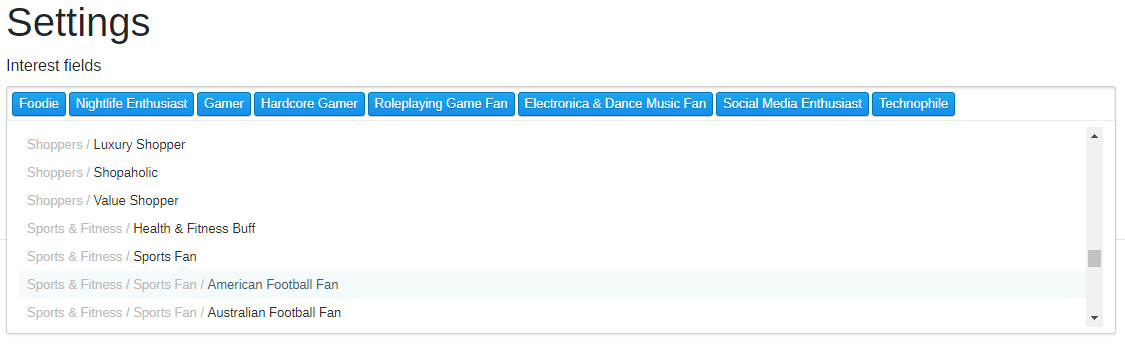
\includegraphics[height=0.32\textwidth]{images/design/pages/settings}
				\caption{Champ d'entrée des centres d'intérêts}
				\label{settings_image}
			\end{figure}

			Un maximum de 10 centres d'intérêts peuvent être définis. Le but de laisser à l'utilisateur entrer des centres d'intérêts est de pouvoir nous rendre compte si les topics que nous lui proposons sont proches de ces centres d'intérêt.

		\subsubsection{Association topic et intérêt}

			Une fois que l'utilisateur a défini des centres d'intérêt, il peut donner des informations sur les topics que nous lui suggérons sur la page Topics List (voir section \ref{topicslist}). La figure~\ref{choice} montre la fenêtre déroulante de sélection d'un centre d'intérêt pour un topic donné.

			\begin{figure}[!h]
				\centering
				
\includegraphics[height=0.32\textwidth]{images/results/choice}
				\caption{Sélection d'intérêt sur un topic}
				\label{choice}
			\end{figure}

			Il est demandé aux utilisateurs d'ajouter une association entre un topic et un intérêt lorsque cela semble lui faire sens. Ainsi, nous pouvons savoir quels topics de l'utilisateur nous avons réussi à identifier. En effet, lorsqu'un utilisateur associe un centre d'intérêt à un topic, celà signifie non seulement que le topic trouvé a du sens en soi, mais en plus qu'il est intéressant pour l'utilisateur.

			Sur l'échantillon de 8 personnes actives, 6 personnes ont ajouté des associations aux 20 topics proposés sur leur page. 

\section{Résultats de la recherche}

	Après une récolte des données sur environ 4 semaines, nous pouvons nous intéresser aux résultats que nous avons récoltés.

	\subsection{Modèles}

		Une première étape est de se pencher sur les modèles que nous avons généré sur la base des données elle-mêmes. Nous utilisons principalement deux algorithmes qui se basent sur le contenu des pages pour en déterminer leur thème : TF-IDF, et LDA.

		\subsubsection{TF-IDF}

			\paragraph{Fonctionnement}

				TF-IDF est une méthode attribuant un poids à chaque mot de chaque document d'un corpus. Ce poids mesure l'importance relative du mot dans ce document. Le nom "TF-IDF" signifie "Term Frequency - Inverse Document Frequency". Le poids final d'un mot dans un document se calcule en prenant en compte uniquement deux mesures :
				\begin{description}
					\item[TF] Term Frequency : La quantité d'apparition de ce mot dans ce document
					\item[DF] Document Frequency : Le nombre de documents dans lequels ce mot apparaît
				\end{description}

				Le score final d'un mot multiplie le TF d'un mot à l'inverse de son DF. Celà signifie que pour avoir une grande importance dans un document, un mot sera typiquement :
				\begin{itemize}
					\item Présent de nombreuses fois dans ce document
					\item Présent dans très peu d'autres documents
				\end{itemize}

				Le calcul des poids se fait sur l'ensemble du corpus, en une fois, car il nécessite que l'on connaisse le nombre d'occurences de chaque mot dans l'entièreté du corpus de documents. Il n'est donc pas possible de mettre à jour les poids de manière "online" en utilisant ce modèle.

			\paragraph{Résultats}

				Juger les résultats du calcul de TF-IDF sur des documents est une tâche non triviale. Cela revient principalement à vérifier manuellement que les mots ayant le poids le plus élevé pour certaines pages soit significatif de leur sujet.

				Intéressons-nous donc aux mots ayant le plus de poids trouvés pour les 20 pages les plus regardées, par exemple. Le tableau\ref{table-tfidf} illustre les 20 pages les plus regardées avec leurs mots associés, ainsi que plusieurs étapes amenant à une estimation finale de l'adéquation des mota trouvés avec le contenu de la page. Voici comment se lit le tableau :
				\begin{description}
					\item[URL] URL de la page concernée. Certaines URLs trop longues ont été raccourcies ici
					\item[Mot 1, 2, 3] 3 meilleurs mots dans l'orrdre décroissant décrivant la page selon TF-IDF.
					\item[Pub(lique)] Est-ce que la page nécessite une connexion afin d'accéder à son contenu principal.
					\item[Con(tenu)] Est-ce que le principal contenu de la page est textuel ?
					\item[Mot] Est-ce que chacun des mots trouvés sur la page fait sens dans une langue connue ?
					\item[Adé(quat)] Est-ce que l'ensemble des mots trouvés forme un potentiel résumé adéquat du contenu de la page ?
				\end{description}

				Les 4 premières colonnes (URL et 3 mots) proviennent de la base de données, tandis que les 4 dernières colonnes sont le résultat d'une évaluation manuelle des critères décrits. Un "OUI" dans une colonne indique que la page a passé le critère défini, contrairement à un "NON". Un "NON" dans une colonne entraîne automatiquement un "NON" dans les colonnes situées les plus à droite.

\begin{sidewaysfigure}
\centering
\caption{20 URLs les plus regardées et leurs meilleurs mots selon TF-IDF}
\label{table-tfidf}
\begin{tabular}{llllllll}
\textbf{URL}                                          & \textbf{Mot 1}  & \textbf{Mot 2}           & \textbf{Mot 3} & \textbf{Pub}           & \textbf{Con}            & \textbf{Mot}               & \textbf{Adé}            \\ \hline
\scriptsize \url{http://wdf.sdipi.ch/}                              & footprints      & digital                  & web            & \cellcolor[HTML]{9AFF99}OUI & \cellcolor[HTML]{9AFF99}OUI & \cellcolor[HTML]{9AFF99}OUI & \cellcolor[HTML]{9AFF99}OUI \\
\scriptsize \url{https://www.draw.io/}                                  & gmdl            & eng                      & proc           & \cellcolor[HTML]{9AFF99}OUI & \cellcolor[HTML]{FFCCC9}NON & \cellcolor[HTML]{FFCCC9}NON & \cellcolor[HTML]{FFCCC9}NON \\
\scriptsize \url{https://www.reddit.com/r/videos/}                      & submit          & load                     & report         & \cellcolor[HTML]{9AFF99}OUI & \cellcolor[HTML]{9AFF99}OUI & \cellcolor[HTML]{9AFF99}OUI & \cellcolor[HTML]{FFCCC9}NON \\
\scriptsize \url{https://www.google.co.uk/search}                       & eingabetaste    & suche                    & drücke         & \cellcolor[HTML]{9AFF99}OUI & \cellcolor[HTML]{FFCCC9}NON & \cellcolor[HTML]{FFCCC9}NON & \cellcolor[HTML]{FFCCC9}NON \\
\scriptsize \url{https://www.google.ch/search}                          & eingabetaste    & suche                    & drücke         & \cellcolor[HTML]{9AFF99}OUI & \cellcolor[HTML]{FFCCC9}NON & \cellcolor[HTML]{FFCCC9}NON & \cellcolor[HTML]{FFCCC9}NON \\
\scriptsize \url{http://game110.idlekiller.com/}                        & explorer        & chrome                   & browser        & \cellcolor[HTML]{9AFF99}OUI & \cellcolor[HTML]{9AFF99}OUI & \cellcolor[HTML]{9AFF99}OUI & \cellcolor[HTML]{9AFF99}OUI \\
\scriptsize \url{http://df.sdipi.ch/phpmyadmin/sql.php}                 & phpmyadmin      & past                     & welcome        & \cellcolor[HTML]{FFCCC9}NON & \cellcolor[HTML]{FFCCC9}NON & \cellcolor[HTML]{FFCCC9}NON & \cellcolor[HTML]{FFCCC9}NON \\
\scriptsize \url{https://web.whatsapp.com/}                             & whatsapp        & macos                    & mozilla        & \cellcolor[HTML]{FFCCC9}NON & \cellcolor[HTML]{FFCCC9}NON & \cellcolor[HTML]{FFCCC9}NON & \cellcolor[HTML]{FFCCC9}NON \\
\scriptsize \url{http://hexaclicker.github.io/}                         & hexa            & dp                       & level          & \cellcolor[HTML]{9AFF99}OUI & \cellcolor[HTML]{9AFF99}OUI & \cellcolor[HTML]{9AFF99}OUI & \cellcolor[HTML]{9AFF99}OUI \\
\scriptsize \url{http://blankmediagames.com/TownOfSalem/}              & salem           & adobe                    & town           & \cellcolor[HTML]{9AFF99}OUI & \cellcolor[HTML]{FFCCC9}NON & \cellcolor[HTML]{FFCCC9}NON & \cellcolor[HTML]{FFCCC9}NON \\
\scriptsize \url{http://www.jeuxvideo.com/}                             & jeu             & annonce                  & bande          & \cellcolor[HTML]{9AFF99}OUI & \cellcolor[HTML]{9AFF99}OUI & \cellcolor[HTML]{9AFF99}OUI & \cellcolor[HTML]{9AFF99}OUI \\
\scriptsize \url{https://discordapp.com/channels/217...408/217...408}   & own             & respective               & owner          & \cellcolor[HTML]{FFCCC9}NON & \cellcolor[HTML]{FFCCC9}NON & \cellcolor[HTML]{FFCCC9}NON & \cellcolor[HTML]{FFCCC9}NON \\
\scriptsize \url{https://www.reddit.com/r/leagueoflegends/}             & leagueoflegends & submit                   & self           & \cellcolor[HTML]{9AFF99}OUI & \cellcolor[HTML]{9AFF99}OUI & \cellcolor[HTML]{9AFF99}OUI & \cellcolor[HTML]{9AFF99}OUI \\
\scriptsize \url{https://www.reddit.com/}                               & bot             & agent                    & pardner        & \cellcolor[HTML]{9AFF99}OUI & \cellcolor[HTML]{9AFF99}OUI & \cellcolor[HTML]{9AFF99}OUI & \cellcolor[HTML]{FFCCC9}NON \\
\scriptsize \url{https://www.google.fr/search}                          & eingabetaste    & suche                    & drücke         & \cellcolor[HTML]{9AFF99}OUI & \cellcolor[HTML]{FFCCC9}NON & \cellcolor[HTML]{FFCCC9}NON & \cellcolor[HTML]{FFCCC9}NON \\
\scriptsize \url{https://s3-fr.gladiatus.gameforge.com/game/index.php}  & de              & gameforge                & vous           & \cellcolor[HTML]{FFCCC9}NON & \cellcolor[HTML]{FFCCC9}NON & \cellcolor[HTML]{FFCCC9}NON & \cellcolor[HTML]{FFCCC9}NON \\
\scriptsize \url{https://docs.google.com/presentation/d/1IB...l5w/edit} & row5w           & gecb...el5w & slide          & \cellcolor[HTML]{FFCCC9}NON & \cellcolor[HTML]{FFCCC9}NON & \cellcolor[HTML]{FFCCC9}NON & \cellcolor[HTML]{FFCCC9}NON \\
\scriptsize \url{https://twitter.com/}                                  & tweet           & foto                     & hast           & \cellcolor[HTML]{9AFF99}OUI & \cellcolor[HTML]{FFCCC9}NON & \cellcolor[HTML]{FFCCC9}NON & \cellcolor[HTML]{FFCCC9}NON \\
\scriptsize \url{http://df.sdipi.ch/phpmyadmin/db\_structure.php}       & phpmyadmin      & past                     & welcome        & \cellcolor[HTML]{FFCCC9}NON & \cellcolor[HTML]{FFCCC9}NON & \cellcolor[HTML]{FFCCC9}NON & \cellcolor[HTML]{FFCCC9}NON \\ \hline
\end{tabular}
\end{sidewaysfigure}

			\paragraph{Réflexion}

				Le tableau~\ref{resultats-tfidf} montre un résumé des résultats que l'on peut récupérer précédent tableau. On remarque que sur les 20 URLs entrées, seules 7 valent vraiment la peine d'être parcourues par notre algorithme, par élimination à causes des deux premières raisons énoncées. Cependant, sur les 7 URLs contenant du texte intéressant, TF-IDF a été capable d'en résumer adéquatement 5 d'entre-elles.

				Ce résultat est loin d'être parfait, mais il montre tout de même qu'il est possible d'automatiser la recherche de mots importants sur des pages lorsque les conditions sont favorables à notre approche.

\FloatBarrier

				\begin{table}[h]
\centering
\caption{Résumé des résultats de TF-IDF}
\label{resultats-tfidf}
\begin{tabular}{lr}
\textbf{URLs initiales}            & 20 \\
\textbf{Pages publiques}           & 14 \\
\textbf{Contenu textuel principal} & 7  \\
\textbf{Mots sensés}               & 7  \\
\textbf{Mots adéquats}             & 5 
\end{tabular}
\end{table}

		\subsubsection{LDA}

			\paragraph{Fonctionnement}

				LDA est un modèle probabiliste, permettant...

			\paragraph{Résultats}

			\paragraph{Réflexion}

	\subsection{Statistiques}

		\subsubsection{Profiling}

		\subsubsection{Trackers}

	\subsection{Implications}

\section{Conclusion}